
%	\addcontentsline{toc}{chapter}{Preface}
	\chapter*{Preface}

%\section*{Organizational stuff}
\begin{itemize}
	\item Questions, comments and suggestions are welcome. Especially, if you find any errors in the lecture notes or if you have difficulties with some contents, please let me know. 
	\item You can contact (at every time) me in the lecture or via 
	\itex{	\item phone (+49 221 973199-523), 
		\item e-mail \texttt{Stephan.Huber@hs-fresenius.de}),
		\item in office, and
		\item online. For making an appointment, you can use the online tool that you find on my private homepage: \url{https://hubchev.github.io/}
	}
	\item Material such as slides and lecture notes can be found on ILIAS, Studynet, Lentera cloud, or my private homepage and GitHub Account.
%	\item Workload: 125 h = 28 h (in-class) + 35 h (guided private study hours) -  62 h (private self-study).
%	\item Students complete this module with a written exam of 90 minutes. A passing grade in this module
%is achieved when the overall grade is greater than or equal to 4.0.
%	\item The students who have successfully completed the module are able to:
%	\itex{
%\item describe the basics of economic reasoning and the concept of scarcity,
%\item discuss the use of the assumption of rationally acting individuals in economic theory,
%\item apply appropriate terminology, concepts, measures, and theories in economic contexts,
%\item analyse the outcomes of consumer and producer decisions in an economy,
%\item predict the consequences of exogenous shocks, and government actions at the aggregate
%level by applying basic economic concepts and theories,
%\item describe the welfare implications of international trade,
%\item identify the nature and causes of contemporary economic problems and issues for
%individuals, firms and governments, and discuss appropriate policies to solve them,
%\item apply mathematical models to international financial products.
%	}
\pbn
	\item 	My teaching principle is \textbf{KISS} which stands for \textbf{keep it simple and straightforward}.

The KISS principle states that most systems work best if they are kept simple rather than complicated; therefore, simplicity should be a key goal in design, and unnecessary complexity should be avoided. 

\boxb{However, KISS does not mean that the course is easy! If you are not able to think logically or if you are not willing to work hard, you may have problems passing the course}

Given your talent and mental capacities, I try to maximize your ability and self-confidence to solve future problems (in life and work).

\item 	I am convinced that reading the lecture notes, preparing for class, taking actively part in class, and trying to solve the exercises without going straight to the solutions is the best method for students to \itex{
	
	\item maximize leisure time and minimize the time needed to prepare for the exam, respectively,
	
	\item getting long-term benefits out of the course, 
	
	\item improve grades, and 
	
	\item have more fun during lecture hours.
	
}
	\pbn
	
	\item \textbf{Literature:}
This lecture just scratches the surface of many economic phenomena. For a deeper
understanding, you should read a textbook. Any major economics textbook can be used
for this lecture. I personally recommend \itex{
		\item \bibentry{Mankiw2020Principles},
		\item \bibentry{Blanchard2013Blanchard},
		\item \bibentry{Shapiro2022Principles}, 
	}
		but you can also use 
\itex{		\item \bibentry{Parkin2012Economics}, {Case2019Principles}, , or 
		\item \bibentry{Krugman2018Economics}.} 
	While it is always nice to have a more recent textbook, basically older copies are just as fine (and much cheaper). Also, there are good books that are freely available online such as 
	\itex{
		\item \bibentry{Shapiro2022Principles}, 
		\item \bibentry{Anonymous2020Principles}, 
		\item \bibentry{Goodwin2012Economix}, and 
		\item \bibentry{Klein2010Cartoon}.
	}


%	\pbn
\item I present international economics divided into three major branches: 
\desx{
	\item[International trade] is concerned with the determination of relative prices and real incomes in international trade abstracting from the intervention of money. That means trade is considered as an exchange of goods with no financial transactions involved. Of course, this assumption is unrealistic. However, it helps to understand the driving forces of real-world problems. 
	\item[Monetary international economics] explicitly considers the meaning of the international financial transaction. 
	\item[International trade policy] is about how international economics is taken into action to build the world we live in.
}
	\item Of course, this lecture cannot cover all aspects of international economics. t's more like a curated collection of crucial concepts to grasp the fundamentals of global trade. For a deeper dive, I suggest exploring a standard international economics textbook of your preference. Below is a list of recommended books::
\itex{
	\item \cite{Academy2012International}: \bibentry{Academy2012International}
	\item \cite{Krugman2017International}: \bibentry{Krugman2017International}
	\item \cite{Feenstra2017International}: \bibentry{Feenstra2017International}
	\item \cite{Pugel2015International}: \bibentry{Pugel2015International}
	\item \cite{Robert2016International}: \bibentry{Robert2016International}
	\item \cite{Marrewijk2012International}: \bibentry{Marrewijk2012International}
	\item \cite{Marrewijk2017International}: \bibentry{Marrewijk2017International}
}
\nocite{Krugman2017International, Feenstra2017International,Pugel2015International, Robert2016International} \nocite{Marrewijk2012International,Marrewijk2017International}

\pbn
\item Plan for an international economics course:

%	\scalebox{1.2}{
	\begin{tabularx}{\textwidth}{r |@{\foo} lX}
		\toprule
		Section & Lecture & Tutorial and/or Self-Study\\\midrule
		1	& Preface, \autoref{ch:econintro}	& \pencil exercises: \ref{exe:Trade and Putin}, \ref{exe:Magic of the price system}, \ref{exe:Free trade: good or bad?}, \ref{exe:A country is not a company} \readsmall \autoref{sec:Important terms (glossary)}	\\
		2		& \autoref{sec:The foreign exchange market}, \autoref{sec:Purchasing power parity assumption}	
		& \pencil exercises: 	\autoref{exe:Arbitrage}, \autoref{exe:Big-Mac-Index vs. Mac-Index}\\
		
		
		3		& \autoref{sec:International investments}	& \pencil exercises: \ref{exe:Big Mac economics}, \ref{exe:Brexit and the exchange rate}, \ref{exe:FOREX MC}, \ref{exe:Turkey vs. Germany}	\\
		4	& \autoref{sec:balance-of-payments}	and \autoref{micro-pre} &	\\
		5	& \autoref{sec:mankiw} -- \autoref{sec:reasons}	& \pencil exercises: \ref{exe:Understanding production}\\
		6	& \autoref{sec:exchange-economy}	& \pencil exercise: \ref{exe:How Barbara and Anton trade},	\ref{exe:Terms of trade}\\
		7	& \autoref{sec:imi}	& \pencil exercises: 	\ref{exe:Terms of trade}, \ref{exe:Production and consumption}, \ref{exe:Gains of small economies}	\\
		%		17 & ----- no lecture	&	\\
		8	& \autoref{sec:ricardo}	&   \pencil exercises: \ref{exe:Indifference curves for perfect complementary goods}	\\
		9	&	&  \pencil exercises:  \ref{exe:Comparative advantage and input coefficients} -- \ref{exe:Bikes and bike tires}	\\
		10	& \autoref{sec:ho}	&  \pencil exercises:  \ref{exe:Ricardian model MC} -- \ref{exe:Multiple choice: HO-Model}	\\
		11	& \autoref{sec:Stylized facts on trade openness} -- \autoref{sec:Trump and trade}	&  \pencil exercises: \ref{exe:Buy local be happy?}, \ref{exe:God's diplomacy}, \ref{exe:Trump complains about the WTO}	\\
		12 	& \autoref{sec:Arguments for trade restrictions} -- \autoref{sec:Other nontariff trade barriers}	&  \pencil exercises:  \ref{exe:Arguments for trade restrictions}, \ref{exe:Tariff}	\\
		13/14	&Exam preparation, Q\&A & \pencil past exams	\\
		%		14	&Mock Exam	&	\\
		
		\bottomrule
	\end{tabularx}

	\item \textbf{Notes on Economic models:}\\
In the following sections, I introduce some mathematical economic models and concepts that are helpful to think about economics in a structured way. Moreover, knowledge on these concepts will allow you to read up-to-date textbooks and literature. Last but not least, the concepts, i.e., formulas and graphical visualizations of arguments can be helpful to understand, analyze, and memorize more complex situations of international trade.

Economic models are based on transparent assumptions and generally consist of a set of equations that describe a theory of economic behavior. A good model should provide useful insights into how rational agents behave and how the economy works. 
Unfortunately, sometimes students feel lost with these models as the models draw on mathematics and rigorous logical thinking. I often hear that there are less sophisticated ways to formulate the argument and that I act like the teacher of \autoref{fig:bozos}. While that may sometimes be true, I am deeply convinced that the formal way to introduce international economics is the best way in the medium and long term. Let me justify my conviction: 
\enux{
	\item The narrative method, i.e., telling stories and listing bullet points, is an efficient way to quickly inform about different types of topics, but it also has drawbacks: Students easily get lost in intuitive-sounding anecdotes without learning to think critically and identify underlying general driving forces. Students tend to cram the information told just for the exam and quickly forget everything afterward. 
	\item  Compared to an anecdote, a formal model is not necessarily true. However, they can provide more insight into a topic than an anecdote or other type of storytelling.
	\item A formal model is usually more flexible compared to stories and anecdotes. Once students understand the underlying logic of a model and are able to interpret and evaluate its meaning, they can apply the findings to a variety of circumstances or problems. An anecdote, on the other hand, is just a story that may represent a limited view of a problem. Overall, drawing general conclusions and analogies from anecdotal evidence is problematic.  
	\item A mathematical economic model is like a proof of an argument. It states exactly under what assumptions an argument is true. In a narrative, it is often difficult to see the underlying assumptions and premises of an argument. 
	\item The formal way of reasoning about things is the standard in economic research, and therefore by knowing the basic concepts, students can read and understand the current literature to do research and solve problems in their professional lives.
	\item Once students understand an economic model, they know the underlying relationships, which they are less likely to forget. In other words, \textbf{a formal model ensures that students are not just repeating the teacher's words, but are able to think and reason for themselves.}
}
\end{itemize}	

\begin{figure}[H]
\begin{center}
	
	\includegraphics[width=.7\linewidth]{$HOME/Dropbox/hsf/pic/soph}
	\caption{How to be a bad teacher of international economics}
	\label{fig:bozos} 
	
\end{center}
\end{figure}

	
\boxb{\subsection*{How to prepare for the exam}\label{sec:howtoprepare}
	\begin{minipage}{0.2\textwidth}
		\includegraphics[width=0.9\linewidth]{../../../pic/Richard-Feynman}
	\end{minipage}
	\begin{minipage}{0.8\textwidth}
		Richard P. Feynman: \zitat{``I don't know what's the matter with people: they don't learn by understanding; they learn by some other way ­­ by rote, or something. Their knowledge is so fragil!''}
	\end{minipage}
	\begin{minipage}{0.2\textwidth}
		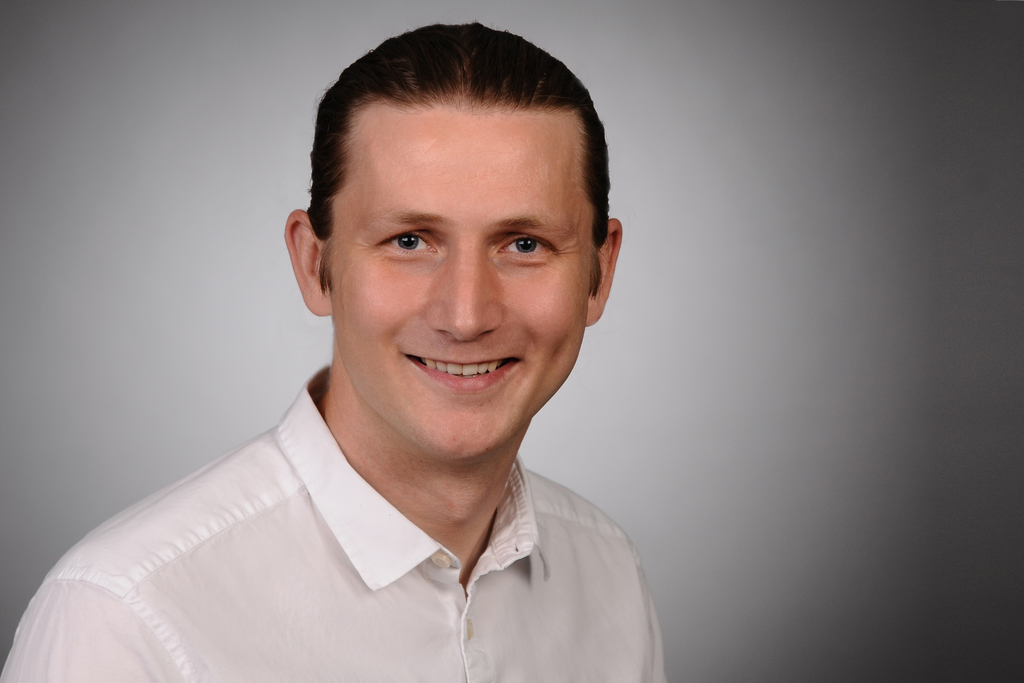
\includegraphics[width=0.9\linewidth]{../../../pic/huber2}
	\end{minipage}
	\begin{minipage}{0.8\textwidth}
		Stephan Huber: \zitat{I agree with Feynman: The key to learning is understanding. However, I believe that there is no understanding without practice, that is, solving problems and exercises by yourself with a pencil and a blank sheet of paper without knowing the solution in advance.}
	\end{minipage}\medskip
	
	\itex{
		\item Study the lecture notes, i.e., try to understand the exercises and solve them yourself. 
		\item Study the exercises, i.e., try to understand the logical rules and solve the problems yourself. 
		\item Test yourself with past exams that you will find online. . 
		\item If you have the opportunity to form a group of students to study and prepare for the exam, make use of it. It is great to help each other, and it is very motivating to see that everyone has problems sometimes.
		\item If you have difficulties with some exercises and the solutions shown do not solve your problem, ask a classmate or contact me. I will do my best to help. 
	}
}
%	\item Module Content
%	\itex{\item Numbers and Equations
%		\item Series, Power Series, Limits, Convergence
%		\item Functions
%		\item Differentiation and Integration
%		\item Vectors and Matrices
%		\item Linear Equation Systems
%		\item Optimization with Constraints: Lagrange Multipliers}

